% Options for packages loaded elsewhere
\PassOptionsToPackage{unicode}{hyperref}
\PassOptionsToPackage{hyphens}{url}
%
\documentclass[
]{book}
\usepackage{amsmath,amssymb}
\usepackage{lmodern}
\usepackage{ifxetex,ifluatex}
\ifnum 0\ifxetex 1\fi\ifluatex 1\fi=0 % if pdftex
  \usepackage[T1]{fontenc}
  \usepackage[utf8]{inputenc}
  \usepackage{textcomp} % provide euro and other symbols
\else % if luatex or xetex
  \usepackage{unicode-math}
  \defaultfontfeatures{Scale=MatchLowercase}
  \defaultfontfeatures[\rmfamily]{Ligatures=TeX,Scale=1}
\fi
% Use upquote if available, for straight quotes in verbatim environments
\IfFileExists{upquote.sty}{\usepackage{upquote}}{}
\IfFileExists{microtype.sty}{% use microtype if available
  \usepackage[]{microtype}
  \UseMicrotypeSet[protrusion]{basicmath} % disable protrusion for tt fonts
}{}
\makeatletter
\@ifundefined{KOMAClassName}{% if non-KOMA class
  \IfFileExists{parskip.sty}{%
    \usepackage{parskip}
  }{% else
    \setlength{\parindent}{0pt}
    \setlength{\parskip}{6pt plus 2pt minus 1pt}}
}{% if KOMA class
  \KOMAoptions{parskip=half}}
\makeatother
\usepackage{xcolor}
\IfFileExists{xurl.sty}{\usepackage{xurl}}{} % add URL line breaks if available
\IfFileExists{bookmark.sty}{\usepackage{bookmark}}{\usepackage{hyperref}}
\hypersetup{
  pdftitle={A Minimal Book Example},
  pdfauthor={Yihui Xie},
  hidelinks,
  pdfcreator={LaTeX via pandoc}}
\urlstyle{same} % disable monospaced font for URLs
\usepackage{color}
\usepackage{fancyvrb}
\newcommand{\VerbBar}{|}
\newcommand{\VERB}{\Verb[commandchars=\\\{\}]}
\DefineVerbatimEnvironment{Highlighting}{Verbatim}{commandchars=\\\{\}}
% Add ',fontsize=\small' for more characters per line
\usepackage{framed}
\definecolor{shadecolor}{RGB}{248,248,248}
\newenvironment{Shaded}{\begin{snugshade}}{\end{snugshade}}
\newcommand{\AlertTok}[1]{\textcolor[rgb]{0.94,0.16,0.16}{#1}}
\newcommand{\AnnotationTok}[1]{\textcolor[rgb]{0.56,0.35,0.01}{\textbf{\textit{#1}}}}
\newcommand{\AttributeTok}[1]{\textcolor[rgb]{0.77,0.63,0.00}{#1}}
\newcommand{\BaseNTok}[1]{\textcolor[rgb]{0.00,0.00,0.81}{#1}}
\newcommand{\BuiltInTok}[1]{#1}
\newcommand{\CharTok}[1]{\textcolor[rgb]{0.31,0.60,0.02}{#1}}
\newcommand{\CommentTok}[1]{\textcolor[rgb]{0.56,0.35,0.01}{\textit{#1}}}
\newcommand{\CommentVarTok}[1]{\textcolor[rgb]{0.56,0.35,0.01}{\textbf{\textit{#1}}}}
\newcommand{\ConstantTok}[1]{\textcolor[rgb]{0.00,0.00,0.00}{#1}}
\newcommand{\ControlFlowTok}[1]{\textcolor[rgb]{0.13,0.29,0.53}{\textbf{#1}}}
\newcommand{\DataTypeTok}[1]{\textcolor[rgb]{0.13,0.29,0.53}{#1}}
\newcommand{\DecValTok}[1]{\textcolor[rgb]{0.00,0.00,0.81}{#1}}
\newcommand{\DocumentationTok}[1]{\textcolor[rgb]{0.56,0.35,0.01}{\textbf{\textit{#1}}}}
\newcommand{\ErrorTok}[1]{\textcolor[rgb]{0.64,0.00,0.00}{\textbf{#1}}}
\newcommand{\ExtensionTok}[1]{#1}
\newcommand{\FloatTok}[1]{\textcolor[rgb]{0.00,0.00,0.81}{#1}}
\newcommand{\FunctionTok}[1]{\textcolor[rgb]{0.00,0.00,0.00}{#1}}
\newcommand{\ImportTok}[1]{#1}
\newcommand{\InformationTok}[1]{\textcolor[rgb]{0.56,0.35,0.01}{\textbf{\textit{#1}}}}
\newcommand{\KeywordTok}[1]{\textcolor[rgb]{0.13,0.29,0.53}{\textbf{#1}}}
\newcommand{\NormalTok}[1]{#1}
\newcommand{\OperatorTok}[1]{\textcolor[rgb]{0.81,0.36,0.00}{\textbf{#1}}}
\newcommand{\OtherTok}[1]{\textcolor[rgb]{0.56,0.35,0.01}{#1}}
\newcommand{\PreprocessorTok}[1]{\textcolor[rgb]{0.56,0.35,0.01}{\textit{#1}}}
\newcommand{\RegionMarkerTok}[1]{#1}
\newcommand{\SpecialCharTok}[1]{\textcolor[rgb]{0.00,0.00,0.00}{#1}}
\newcommand{\SpecialStringTok}[1]{\textcolor[rgb]{0.31,0.60,0.02}{#1}}
\newcommand{\StringTok}[1]{\textcolor[rgb]{0.31,0.60,0.02}{#1}}
\newcommand{\VariableTok}[1]{\textcolor[rgb]{0.00,0.00,0.00}{#1}}
\newcommand{\VerbatimStringTok}[1]{\textcolor[rgb]{0.31,0.60,0.02}{#1}}
\newcommand{\WarningTok}[1]{\textcolor[rgb]{0.56,0.35,0.01}{\textbf{\textit{#1}}}}
\usepackage{longtable,booktabs,array}
\usepackage{calc} % for calculating minipage widths
% Correct order of tables after \paragraph or \subparagraph
\usepackage{etoolbox}
\makeatletter
\patchcmd\longtable{\par}{\if@noskipsec\mbox{}\fi\par}{}{}
\makeatother
% Allow footnotes in longtable head/foot
\IfFileExists{footnotehyper.sty}{\usepackage{footnotehyper}}{\usepackage{footnote}}
\makesavenoteenv{longtable}
\usepackage{graphicx}
\makeatletter
\def\maxwidth{\ifdim\Gin@nat@width>\linewidth\linewidth\else\Gin@nat@width\fi}
\def\maxheight{\ifdim\Gin@nat@height>\textheight\textheight\else\Gin@nat@height\fi}
\makeatother
% Scale images if necessary, so that they will not overflow the page
% margins by default, and it is still possible to overwrite the defaults
% using explicit options in \includegraphics[width, height, ...]{}
\setkeys{Gin}{width=\maxwidth,height=\maxheight,keepaspectratio}
% Set default figure placement to htbp
\makeatletter
\def\fps@figure{htbp}
\makeatother
\setlength{\emergencystretch}{3em} % prevent overfull lines
\providecommand{\tightlist}{%
  \setlength{\itemsep}{0pt}\setlength{\parskip}{0pt}}
\setcounter{secnumdepth}{5}
\usepackage{booktabs}
\ifluatex
  \usepackage{selnolig}  % disable illegal ligatures
\fi
\usepackage[]{natbib}
\bibliographystyle{apalike}

\title{A Minimal Book Example}
\author{Yihui Xie}
\date{2022-02-08}

\usepackage{amsthm}
\newtheorem{theorem}{Theorem}[chapter]
\newtheorem{lemma}{Recipe}[chapter]
\newtheorem{corollary}{Corollary}[chapter]
\newtheorem{proposition}{Proposition}[chapter]
\newtheorem{conjecture}{Conjecture}[chapter]
\theoremstyle{definition}
\newtheorem{definition}{Definition}[chapter]
\theoremstyle{definition}
\newtheorem{example}{Example}[chapter]
\theoremstyle{definition}
\newtheorem{exercise}{Exercise}[chapter]
\theoremstyle{definition}
\newtheorem{hypothesis}{Hypothesis}[chapter]
\theoremstyle{remark}
\newtheorem*{remark}{Remark}
\newtheorem*{solution}{Solution}
\begin{document}
\maketitle

{
\setcounter{tocdepth}{1}
\tableofcontents
}
\hypertarget{prerequisites}{%
\chapter{Prerequisites}\label{prerequisites}}

This is a \emph{sample} book written in \textbf{Markdown}. You can use anything that Pandoc's Markdown supports, e.g., a math equation \(a^2 + b^2 = c^2\).

The \textbf{bookdown} package can be installed from CRAN or Github:

\begin{Shaded}
\begin{Highlighting}[]
\FunctionTok{install.packages}\NormalTok{(}\StringTok{"bookdown"}\NormalTok{)}
\CommentTok{\# or the development version}
\CommentTok{\# devtools::install\_github("rstudio/bookdown")}
\end{Highlighting}
\end{Shaded}

Remember each Rmd file contains one and only one chapter, and a chapter is defined by the first-level heading \texttt{\#}.

To compile this example to PDF, you need XeLaTeX. You are recommended to install TinyTeX (which includes XeLaTeX): \url{https://yihui.org/tinytex/}.

\hypertarget{intro}{%
\chapter{Introduction}\label{intro}}

You can label chapter and section titles using \texttt{\{\#label\}} after them, e.g., we can reference Chapter \ref{intro}. If you do not manually label them, there will be automatic labels anyway, e.g., Chapter \ref{methods}.

Figures and tables with captions will be placed in \texttt{figure} and \texttt{table} environments, respectively.

\begin{Shaded}
\begin{Highlighting}[]
\FunctionTok{par}\NormalTok{(}\AttributeTok{mar =} \FunctionTok{c}\NormalTok{(}\DecValTok{4}\NormalTok{, }\DecValTok{4}\NormalTok{, .}\DecValTok{1}\NormalTok{, .}\DecValTok{1}\NormalTok{))}
\FunctionTok{plot}\NormalTok{(pressure, }\AttributeTok{type =} \StringTok{\textquotesingle{}b\textquotesingle{}}\NormalTok{, }\AttributeTok{pch =} \DecValTok{19}\NormalTok{)}
\end{Highlighting}
\end{Shaded}

\begin{figure}

{\centering 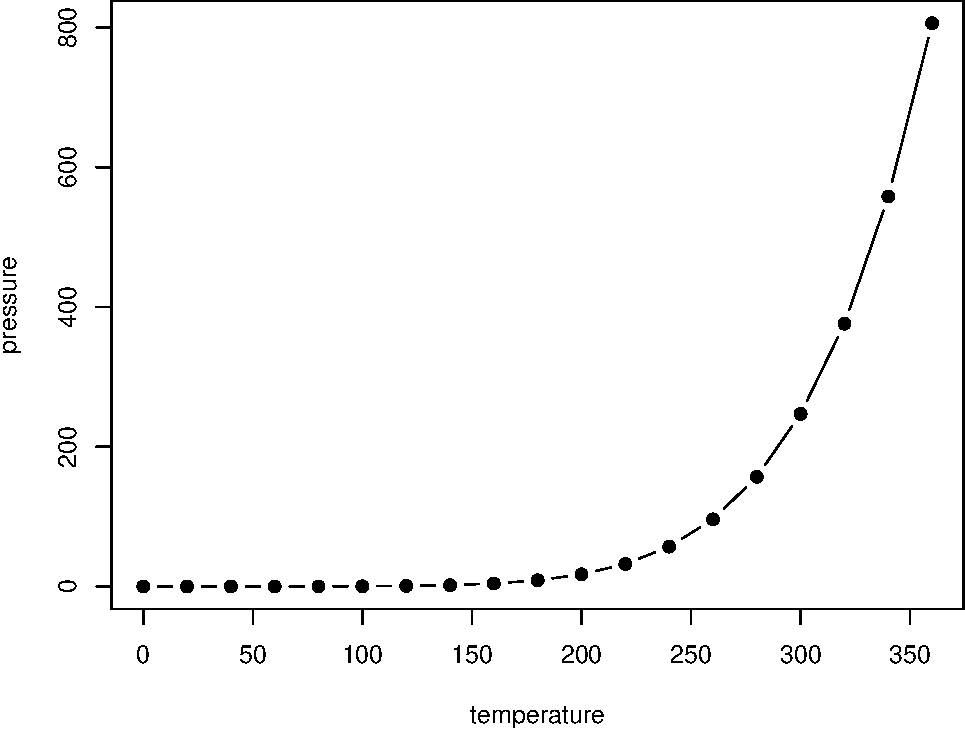
\includegraphics[width=0.8\linewidth]{dollar_dollar_files/figure-latex/nice-fig-1} 

}

\caption{Here is a nice figure!}\label{fig:nice-fig}
\end{figure}

Reference a figure by its code chunk label with the \texttt{fig:} prefix, e.g., see Figure \ref{fig:nice-fig}. Similarly, you can reference tables generated from \texttt{knitr::kable()}, e.g., see Table \ref{tab:nice-tab}.

\begin{Shaded}
\begin{Highlighting}[]
\NormalTok{knitr}\SpecialCharTok{::}\FunctionTok{kable}\NormalTok{(}
  \FunctionTok{head}\NormalTok{(iris, }\DecValTok{20}\NormalTok{), }\AttributeTok{caption =} \StringTok{\textquotesingle{}Here is a nice table!\textquotesingle{}}\NormalTok{,}
  \AttributeTok{booktabs =} \ConstantTok{TRUE}
\NormalTok{)}
\end{Highlighting}
\end{Shaded}

\begin{table}

\caption{\label{tab:nice-tab}Here is a nice table!}
\centering
\begin{tabular}[t]{rrrrl}
\toprule
Sepal.Length & Sepal.Width & Petal.Length & Petal.Width & Species\\
\midrule
5.1 & 3.5 & 1.4 & 0.2 & setosa\\
4.9 & 3.0 & 1.4 & 0.2 & setosa\\
4.7 & 3.2 & 1.3 & 0.2 & setosa\\
4.6 & 3.1 & 1.5 & 0.2 & setosa\\
5.0 & 3.6 & 1.4 & 0.2 & setosa\\
\addlinespace
5.4 & 3.9 & 1.7 & 0.4 & setosa\\
4.6 & 3.4 & 1.4 & 0.3 & setosa\\
5.0 & 3.4 & 1.5 & 0.2 & setosa\\
4.4 & 2.9 & 1.4 & 0.2 & setosa\\
4.9 & 3.1 & 1.5 & 0.1 & setosa\\
\addlinespace
5.4 & 3.7 & 1.5 & 0.2 & setosa\\
4.8 & 3.4 & 1.6 & 0.2 & setosa\\
4.8 & 3.0 & 1.4 & 0.1 & setosa\\
4.3 & 3.0 & 1.1 & 0.1 & setosa\\
5.8 & 4.0 & 1.2 & 0.2 & setosa\\
\addlinespace
5.7 & 4.4 & 1.5 & 0.4 & setosa\\
5.4 & 3.9 & 1.3 & 0.4 & setosa\\
5.1 & 3.5 & 1.4 & 0.3 & setosa\\
5.7 & 3.8 & 1.7 & 0.3 & setosa\\
5.1 & 3.8 & 1.5 & 0.3 & setosa\\
\bottomrule
\end{tabular}
\end{table}

You can write citations, too. For example, we are using the \textbf{bookdown} package \citep{R-bookdown} in this sample book, which was built on top of R Markdown and \textbf{knitr} \citep{xie2015}.

\hypertarget{phylogenetic-birth-death-models}{%
\chapter*{Phylogenetic birth-death models}\label{phylogenetic-birth-death-models}}
\addcontentsline{toc}{chapter}{Phylogenetic birth-death models}

Equations from the litterature to describe birth-death processes in the context of phylogenetic (time)trees.

\hypertarget{louca}{%
\section{\texorpdfstring{\citet{louca_extant_2020} \{-\}}{@louca\_extant\_2020 \{-\}}}\label{louca}}

Number of species predicted at any point in time in a deterministic version of a birth-death process, i.e.~the expected number of species over time in the stochastic process.

We note:

\begin{itemize}
\tightlist
\item
  \(\lambda\) and \(\mu\) the birth and death rate resp., which can be time-dependent (\(\lambda(t)\), \(\mu(t)\))
\item
  \(\rho\) the sampling fraction \emph{at present}, such that \(M_0 = N_0 \rho\) is the number of species sampled in the present tree (and \(N_0\) is the total \textbf{living} diversity)
\end{itemize}

Going backwards in time (\(\tau\) is some time before present):

\begin{align}
  \frac{dN}{d\tau} &= N(\mu - \lambda) \\
   &= N(-r) \label{eq:nbackwards}
\end{align}

The solution of which is (perform a separation of variables):

\begin{align}
  N(\tau) &= N_{0}e^{\left[ \int_0^\tau \mu(u) - \lambda(u) du \right]} \label{eq:nbalive}
\end{align}

i.e.~the number of species alive (but not necessarily sampled in the tree) at time \(\tau\) in the past.

Let's introduce \(E(\tau)\), the fraction of lineages alive at time \(\tau\) that won't be included in the final tree, because of either extinction or being missing from the sample. In a stochastic setting, it is also the probability that a single lineage will be missing from the final tree. \(E(\tau)\) is introduced in \citet{morlon_reconciling_2011}, eqs. 5-7 (where it is named \(\phi(t)\)) (see also the derivation below):

\begin{align}
\frac{dE}{d\tau} &= \mu - E(\lambda - \mu) + E^2\lambda \\
E(0) &= 1 - \rho 
\label{eq:fracmissing}
\end{align}

Its solution is (eq. 2 in \citet{morlon_reconciling_2011}):

\[
E(\tau) = 1 - \frac{e^{\int_0^\tau \lambda(u) - \mu(u) du}}{\frac{1}{f} + \int_0^\tau e^{\int_0^s \lambda(u) - \mu(u) du} \lambda_s ds} 
\label{eq:fracmissingsol}
\]

where \(s\) is some time before \(\tau\), and \(f\) is the probability that a lineage is sampled.

The deterministic LTT, i.e.~the number of lineages present in the final tree, through time, is (by definition of \(M\) and \(E\)) given by:

\[
M(\tau) = N(\tau)(1 - E(\tau)) 
\label{eq:dltt}
\]

Taking the derivative and replacing with \eqref{eq:nbackwards} and \eqref{eq:fracmissing} yields

\[
  \frac{dM}{d\tau} = M\lambda(E-1)
  \label{eq:dlttderiv}
\]
which solution (taking \(M(0) = M_0\) and using a separation of variables) is:

\[
  M(\tau) = M_0e^{\int_0^\tau \lambda(u) (E(u) - 1) du}
  \label{eq:dltt2}
\]
This equation fully describes the LTT expected given the birth-death model, aka the \textbf{dLTT}.

\textbf{Some observations:}

\begin{itemize}
\tightlist
\item
  All terms in this equation are independent of the data! So model congruency (sharing the same dLTT) is a property of the models alone.
\item
  Extinction does not appear in \eqref{eq:dltt2}, but is in fact hidden in \(E(\tau)\)
\item
  In @ref(eq:dltt\_deriv), \(0<E<1\), so that the rhs is negative or zero: we move backwards in time and lose lineages in the phylogeny, proportionally to rate \(\lambda\). The term \(\lambda(E-1)\) (``growth'' rate) can be developped into \(\lambda E - \lambda\), illustrating that we are gaining lineages that would disappear later in time, and losing those that speciate later.
\end{itemize}

\hypertarget{morlon-2011}{%
\section{\texorpdfstring{\citet{morlon_reconciling_2011} \{-\}}{@morlon\_reconciling\_2011 \{-\}}}\label{morlon-2011}}

\hypertarget{derive-e}{%
\subsection{\texorpdfstring{Derivation of \(E(\tau)\) equations \{-\}}{Derivation of E(\textbackslash tau) equations \{-\}}}\label{derive-e}}

\(E(\tau)\) (or \(\Phi(t)\) in \citet{morlon_reconcling_2011}) denotes the probability that a lineage alive at \(\tau\) won't have any descendant included in the final tree.

There are three main combinations of events that can lead to a lineage not having descendants in the final tree:
1. Lineage goes extinct (with probability \(\mu(\tau)\) in a single time unit)
2. No extinction (\(1 - \mu(\tau)\)), no speciation (\(1 - \lambda(\tau)\)), lineage not observed at present (\(E(\tau)\)).
3. No extinction (\(1 - \mu(\tau)\)), lineage undergoes speciation (\(\lambda(\tau)\)) but neither parent or daughter are observed at present (\(E(\tau) * E(\tau)\)).

From this the following recursion can be written:

\begin{align}
  E(\tau + 1) &= \mu \\
  & + (1 - \mu(\tau))(1 - \lambda(\tau)) E(\tau) \\
  & + (1 - \mu(\tau)) \lambda(\tau) E(\tau)^2 \\
  & + o(\tau)
\end{align}

More complex series of events (e.g.~multiple speciation events followed by extinction or non-sampling) are assumed very unlikely to happen in the typical time intervals and rates considered; and thus ignored (\(o(\tau)\).

Deriving an ODE from this recursion goes as follows (see \ref{discrete-to-continuous}:

\$\$
\begin{align}
  E(\tau + \Delta \tau) &= \mu\Delta \tau \\
  & + (1 - \mu(\tau)\Delta \tau)(1 - \lambda(\tau)\Delta \tau) E(\tau) \\
  & + (1 - \mu(\tau)\Delta \tau) \lambda(\tau)\Delta \tau E(\tau)^2 \\
  
  E(\tau + \Delta \tau) - E(\tau) &= \mu\Delta \tau \\
  & - (\lambda + \mu + \lambda \mu \Delta \tau^2) \Delta \tau E(\tau) \\
  & + (1 - \mu(\tau)\Delta \tau) \lambda(\tau)\Delta \tau E(\tau)^2 \\

  \frac{E(\tau + \Delta \tau) - E(\tau)}{\Delta\tau} &= \mu \\
  & - (\lambda + \mu + \lambda \mu \Delta \tau^2) E(\tau) \\
  & + (1 - \mu(\tau)\Delta \tau) \lambda(\tau) E(\tau)^2
  \\

\lim_{\Delta\tau \to 0} \frac{E(\tau + \Delta \tau) - E(\tau)}{\Delta\tau} &= \mu \\
  & - (\lambda + \mu) E(\tau) \\
  & + \lambda(\tau) E(\tau)^2
  \\

\frac{dE}{d\tau} &= \mu - (\lambda + \mu) E(\tau) + \lambda(\tau) E(\tau)^2

\end{align}
\$\$

Note that \citet{morlon_reconciling_2011} made a mistake in eq. 6 and forgot to multiply \(\lambda(t)\) by \(\Delta t\).

We also now that \(E(0) = 1 - \rho\).

\hypertarget{otto-day}{%
\chapter{Otto \& Day shortcuts \{-\}}\label{otto-day}}

Recipes and reading notes from \citet{otto_biologists_2007}.

\hypertarget{discrete-to-continuous}{%
\section{Derive a continuous model from a discrete model \{-\}}\label{discrete-to-continuous}}

Box 2.6, p.44 in \citet{otto_biologists_2007}.

Consider this discrete population growth model, with birth, death and migration:

\[
  n(t+1) = (1 + b)(1-d)n(t) + m
\]

\begin{enumerate}
\def\labelenumi{\arabic{enumi}.}
\tightlist
\item
  Shrink the length of the interval \(t+1\) to something smaller, \(t+\Delta t\).
  Scale down all quantities that scale with time.
  \[
    n(t+\Delta t) = (1 + b\Delta t)(1-d\Delta t)n(t) + m\Delta t
  \]
  \(b\), \(d\), and \(m\) are the number of births, deaths and migrants in a single
  time step. The number that happens during \(t+\Delta t\) is a fraction \(\Delta t\).
\item
  Substract \(n(t)\) from both sides to get \(n(\Delta t)\)
\item
  Divide both sides by \(\Delta t\). Find a way to get \(\Delta t\) out of the denominator.
\item
  Shrink \(\Delta t\), taking the limit \(\lim_{\Delta t\to 0}\)
  \[
    \frac{dn(t)}{dt} = \lim_{\Delta t \to 0} \frac{n(t + \Delta t) - n(t)}{\Delta t}
  \]
\end{enumerate}

For the above example:

\begin{align}
  \frac{n(t + \Delta t) - n(t)}{\Delta t} &= \frac{(1 + b\Delta t)(1 - d\Delta t) + m\Delta t - n(t)}{\Delta t} \\
  &= bn(t) - dn(t) + m -bdn(t)\Delta t
\end{align}

The last term drops when \(\Delta t\) shrinks to 0, yielding:

\[
  \frac{dn(t)}{dt} = (b - d)n(t) + m
\]

\hypertarget{sol}{%
\section{General solution of a model \{-\}}\label{sol}}

\hypertarget{sol-lin-cont-single}{%
\subsection{Linear models, continuous time, single variable \{-\}}\label{sol-lin-cont-single}}

\begin{lemma}[Solving Differential Equations Using a Separation of Variables]
\protect\hypertarget{lem:sepvar}{}{\label{lem:sepvar} \iffalse (Solving Differential Equations Using a Separation of Variables) \fi{} }Differential equations that can be written as \(dn/dt = f(n) g(t)\) can be solved as follows:

\begin{enumerate}
\def\labelenumi{\arabic{enumi}.}
\tightlist
\item
  Define what are \(f(n)\) and \(g(t)\)
\item
  \(\frac{1}{f(n)}dn = g(t)dt\)
\item
  \(\int \frac{1}{f(n)}dn = \int g(t)dt\)
\item
  Solve and don't forget the constants of integration on both sides.
  Lump them together on one side (\(c = c_1-c_2\)).
  Set \(t=0\) or \(N=0\) to find the value of \(c\).
  \end{lemma}
\end{enumerate}

Shortcut: the exponential growth model

\begin{align}
  \frac{dN}{dt} &= rN \\
  N(t) = N_0 e^{rt}
\end{align}

\textbf{Checks}: take the solution and derive to find the differential equation. Use \(N_0\) to replace the exponential term by some function of \(N(t)\).

\textbf{Example} with the affine function \(\frac{dN}{dt} = rN + m\)

Setting \(f(N) = rN + m\) and \(g(t) = 1\).

\[
\begin{align}
  \int \frac{1}{rN + m} dn &= \int 1 dt
\end{align}
\]

I use rule A2.22 in Otto \& Day to solve the lhs, setting \(a_1 = m\), \(b_1 = r\), \(a_2 = 1\) and \(b_2 = 0\).

\[
\begin{align}
  \frac{1}{r} ln(|rN + m|) + cst_1 &= t + cst_2 \\
   ln(|rN + m|) &= r(t + cst) \\
   N(t) &= \frac{1}{r}(e^{r(t + cst)} - m)
\end{align}
\]

Setting \(t=0\) to solve for the \(cst\)

\[
\begin{align}
  N(0) &= \frac{1}{r}(e^{r cst} - m) \\
  cst  &= \frac{1}{r} ln(r N_{0} + m)
\end{align}
\]

So

\[
\begin{align}
   n(t) &= \frac{1}{r}\{e^{r(t)}(rN_0 + m) - m)\} \\
   &= N_0e^{rt} + \frac{m}{r}e^{rt} - \frac{m}{r}
\end{align}
\]

First check: with \(t = 0\), I find \(N(0) = N_0\).

Second check: deriving with respect to \(t\):

\[
\begin{align}
   \frac{dN}{dt} &= (N_0e^{rt})' + \Big(\frac{m}{r}e^{rt}\Big)' - \Big(\frac{m}{r}\Big)' \\
   &= rN_0e^{rt} + me^{rt} \\
   &= r\Big(N_0e^{rt} + \frac{m}{r}e^{rt}\Big) \\
   &= r\Big(N(t) + \frac{m}{r}\Big) \\
   &= rN(t) + m
\end{align}
\]

\hypertarget{applications}{%
\chapter{Applications}\label{applications}}

Some \emph{significant} applications are demonstrated in this chapter.

\hypertarget{example-one}{%
\section{Example one}\label{example-one}}

\hypertarget{example-two}{%
\section{Example two}\label{example-two}}

\hypertarget{final-words}{%
\chapter{Final Words}\label{final-words}}

We have finished a nice book.

  \bibliography{dollar.bib,book.bib,packages.bib}

\end{document}
